\documentclass{exam}
\usepackage[utf8]{inputenc}
\usepackage{lmodern}
\usepackage{microtype}

% \usepackage[parfill]{parskip}
\usepackage[dvipsnames]{xcolor}
\usepackage{amsmath}
\usepackage{amsfonts}
\usepackage{amsthm}
\usepackage{siunitx}
\DeclareSIUnit\year{yr}
\DeclareSIUnit\foot{ft}
\DeclareSIUnit\litre{\liter}

\usepackage{skull}

\usepackage{pgfplots}
\usepgfplotslibrary{polar}
\pgfplotsset{compat=1.11}
\usepgfplotslibrary{statistics}
\usepackage{graphicx}
\usepackage{sidecap}
\sidecaptionvpos{figure}{c}
\usepackage{float}
\usepackage{gensymb}
\usepackage{tkz-euclide}
\usetkzobj{all}
\usepackage{commath}
\usepackage{hyperref}
\usepackage{enumitem}
\usepackage{wasysym}
\usepackage{multicol}
\usepackage{mathtools}
\usepackage{tcolorbox}
\usepackage{tabularx}
\usepackage[version=4]{mhchem}
\usepackage{changepage}
\usepackage{listings}
\lstset{basicstyle=\ttfamily\linespread{0.8}\small}

\renewcommand*{\thefootnote}{\fnsymbol{footnote}}

\newtheorem*{thm}{Theorem}
\newtheorem*{iden}{Identity}
\newtheorem*{lemma}{Lemma}
\newtheorem{obs}{Observation}
\theoremstyle{definition}
\newtheorem*{defn}{Definition}
\newtheorem*{ex}{Example}
\newtheorem{con}{Construction}
\newtheorem*{alg}{Algorithm}

\newtheoremstyle{break}
  {\topsep}{\topsep}%
  {\itshape}{}%
  {\bfseries}{}%
  {\newline}{}%
\theoremstyle{break}
\newtheorem*{bthm}{Theorem}

% russian integral
\usepackage{scalerel}
\DeclareMathOperator*{\rint}{\scalerel*{\rotatebox{17}{$\!\int\!$}}{\int}}

% \DeclareMathOperator*{\rint}{\int}

\pgfplotsset{vasymptote/.style={
    before end axis/.append code={
        \draw[densely dashed] ({rel axis cs:0,0} -| {axis cs:#1,0})
        -- ({rel axis cs:0,1} -| {axis cs:#1,0});
    }
}}

% \pointsinrightmargin
\boxedpoints
\pointname{}

\newcommand{\questioA}{\question[\texttt{\textbf{\color{Cerulean} A}}]}
\newcommand{\questioM}{\question[\texttt{\textbf{\color{PineGreen} M}}]}
\newcommand{\questioE}{\question[\texttt{\textbf{\color{WildStrawberry} E}}]}
\newcommand{\questioS}{\question[\texttt{\textbf{\color{Goldenrod} S}}]}
\newcommand{\questioO}{\question[\texttt{\textbf{\color{BurntOrange} O}}]}

\newcommand{\parA}{\part[\texttt{\textbf{\color{Cerulean} A}}]}
\newcommand{\parM}{\part[\texttt{\textbf{\color{PineGreen} M}}]}
\newcommand{\parE}{\part[\texttt{\textbf{\color{WildStrawberry} E}}]}
\newcommand{\parS}{\part[\texttt{\textbf{\color{Goldenrod} S}}]}
\newcommand{\parO}{\part[\texttt{\textbf{\color{BurntOrange} O}}]}

\newcommand{\subparA}{\subpart[\texttt{\textbf{\color{Cerulean} A}}]}
\newcommand{\subparM}{\subpart[\texttt{\textbf{\color{PineGreen} M}}]}
\newcommand{\subparE}{\subpart[\texttt{\textbf{\color{WildStrawberry} E}}]}
\newcommand{\subparS}{\subpart[\texttt{\textbf{\color{Goldenrod} S}}]}
\newcommand{\subparO}{\subpart[\texttt{\textbf{\color{BurntOrange} O}}]}

\newcommand{\mainHeader}[2]{\section*{NCEA Level 2 Mathematics\\#1. #2}}
\newcommand{\mainHeaderHw}[2]{\section*{NCEA Level 2 Mathematics (Homework)\\#1. #2}}
\newcommand{\seealso}[1]{\begin{center}\emph{See also #1.}\end{center}}
\newcommand{\drills}[1]{\begin{center}\emph{Drill problems: #1.}\end{center}}
\newcommand{\basedon}[1]{\begin{center}\emph{Notes largely based on #1.}\end{center}}

\begin{document}

\mainHeaderDiff{12}{Parametric Functions}
\goals{To understand how calculus can be used to understand the geometry of a path through space.}
\begin{center}
  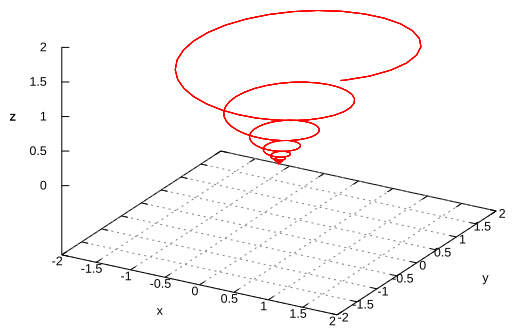
\includegraphics[width=0.5\textwidth]{space-curve-4}
\end{center}
Some curves cannot be described simply with a function; for example, the above track of a particle is
too complicated to analyse using any of the techniques which we have studied so far. One strategy which
does work is to split the $ x $, $ y $, and $ z $ components apart and study them seperately. For
example, we can \textbf{parameterise} the above curve as:
\begin{align*}
  x(t) &= e^{-t} \cos(10t)\\
  y(t) &= e^{-t} \sin(10t)\\
  z(t) &= e^{-t}.
\end{align*}

With this example as our initial motivation, we move from discussing functions $ \mathbb{R} \rightarrow \mathbb{R} $, and turn our attention to
functions $ \mathbb{R} \rightarrow \mathbb{R}^n $. This type of function is often called a \textbf{curve}; a set of component functions, like the
one given above for the spiral, is called a \textbf{parameterisation}.

For a simpler example, consider the unit circle $ x^2 + y^2 = 1 $. By recalling the definitions
of the trigonometric functions, we can parameterise the circle as $ (x, y) = (\cos \theta, \sin \theta) $
for $ 0 \leq \theta < 2\pi $. Then $ \od{y}{t} = -\cos \theta = -x $ and $ \od{x}{t} = \sin \theta = y $,
so by the chain rule $ \od{y}{x} = \od{y}{t} \cdot \od{t}{x} = -\frac{x}{y} $ --- a much simpler calculation
than taking the derivative of the square root required by working directly with the circle formula.

\begin{center}
  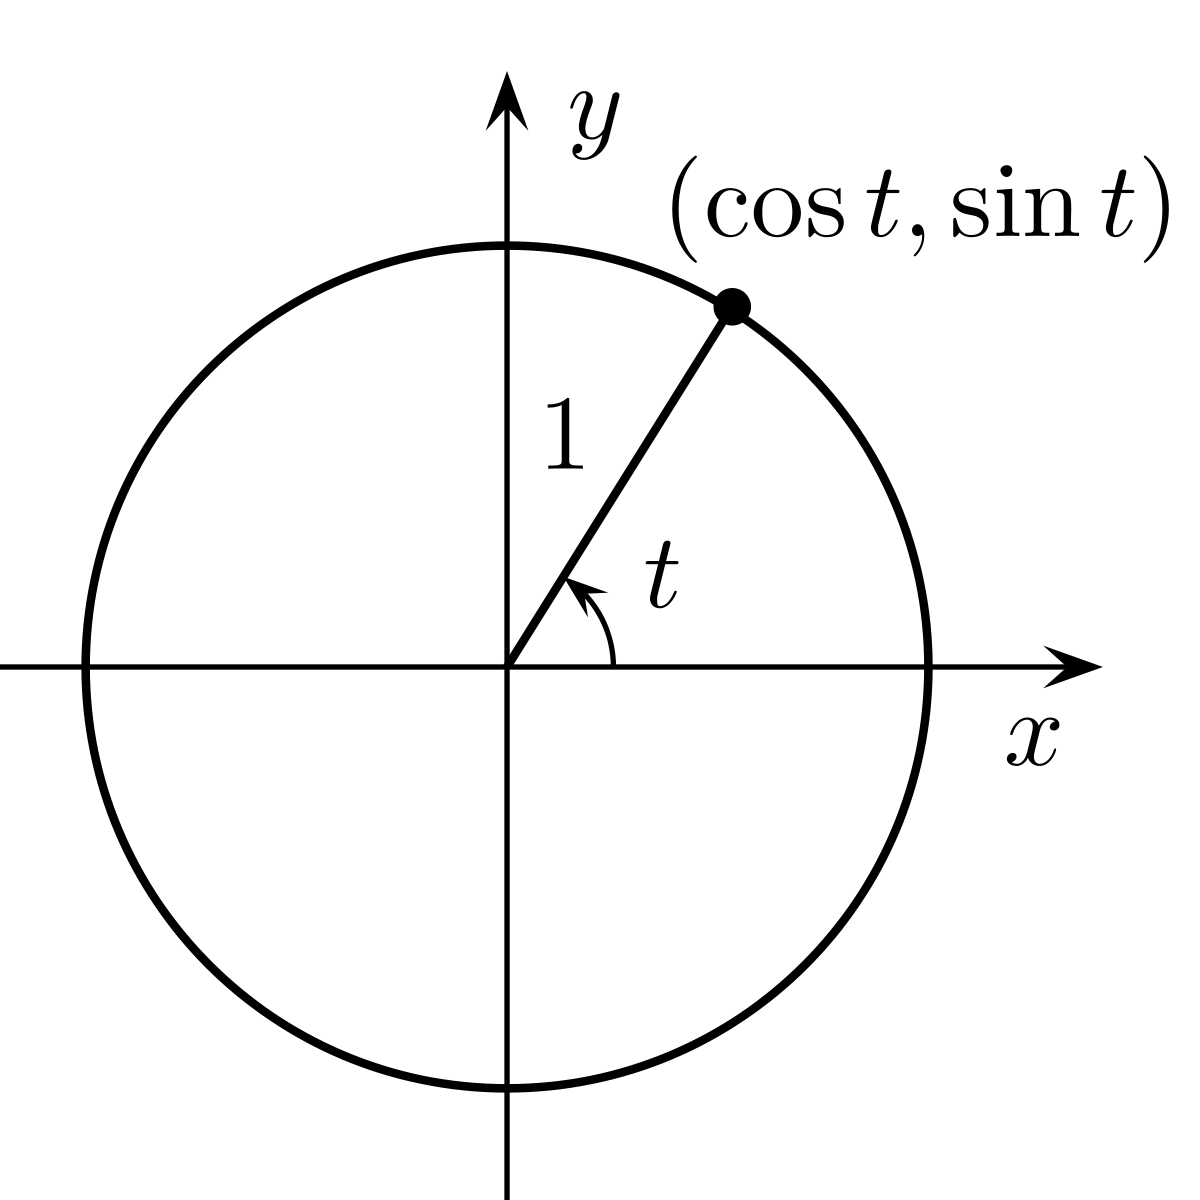
\includegraphics[width=0.2\textwidth]{circle}
\end{center}

In order to justify this in general, we note that the output of a curve is a set of ordered pairs and is therefore (locally) a function from the
first coordinate to the second coordinate. Suppose that we have some curve that is parametrised by $ (x,y) = (f(t), g(t)) $. Then $ y = g(f^{-1}(x)) $ and so
\begin{displaymath}
  \od{y}{x} = \frac{1}{f'(f^{-1}(x))} \cdot g'(f^{-1}(x)) = \frac{1}{f'(t)} \cdot g'(t) = \frac{1}{\od{x}{t}} \cdot \od{y}{t} = \od{y}{t} \cdot \od{t}{x}.
\end{displaymath}

In order to find the second derivative, we replace $ y $ with $ \od{y}{x} $:
\begin{displaymath}
  \dod[2]{y}{x} = \dod{\od{y}{x}}{x} = \left(\dod{}{t} \dod{y}{x}\right) \cdot \dod{t}{x}.
\end{displaymath}

\clearpage
\subsection*{Questions}
\begin{questions}
  \questioM In each case find $ \od{y}{x} $.
    \begin{parts}
      \part $ x = t\sin t $, $ y = t^2 + t $
      \part $ x = 2 \sec \theta $, $ y = 3\tan \theta $
      \part $ x = \cos \theta $, $ y = \cos 3\theta $
      \part $ x = e^{\sin \theta} $, $ y = e^{\cos \theta} $
    \end{parts}
  \questioA Find the equation of the chord joining the two points $ t = 2 $ and $ t = 4 $ on the
            curve $ (x,y) = (2t - 3, t^3 + 6) $.
  \questioM Determine the point(s) of intersection of the curves $ \gamma $ and $ \delta $:
            \begin{align*}
              \gamma &: t \mapsto (t^2 - 2, t - 1)\\
              \delta &: t \mapsto (t, 2/t)
            \end{align*}
  \question
    \begin{parts}
      \parM If $ y = 2t $ and $ x = 4t^2 $ define a curve, what is the gradient $ \od{y}{x} $ in terms of $ t $?
      \parE Show that this curve is a parabola.
    \end{parts}
  \questioM A curve has parametric equations $ x = t^2 + 1 $ and $ y = t^3 + 2 $. Find $ \od{y}{x} $ and $ \od[2]{y}{x} $.
  \questioM Find the equation of the tangent to the curve $ t \mapsto (2x^2 + 1, t^3 - 1) $ at $ t = 2 $.
  \questioE If $ t \mapsto (x, y) $ is a parametric curve, find an expression for $ \od[3]{y}{x} $ analagous to that found for
            the second derivative.
  \questioS A curve, called a \textit{witch of Maria Agnesi}, consists of all possible positions of the point $ P $ in
            the diagram below. Show that the curve is given by $ (x, y) = (2a \cot \theta, 2a \sin^2 \theta) $ and
            find the derivative $ \od{y}{x} $.
            \begin{center}
              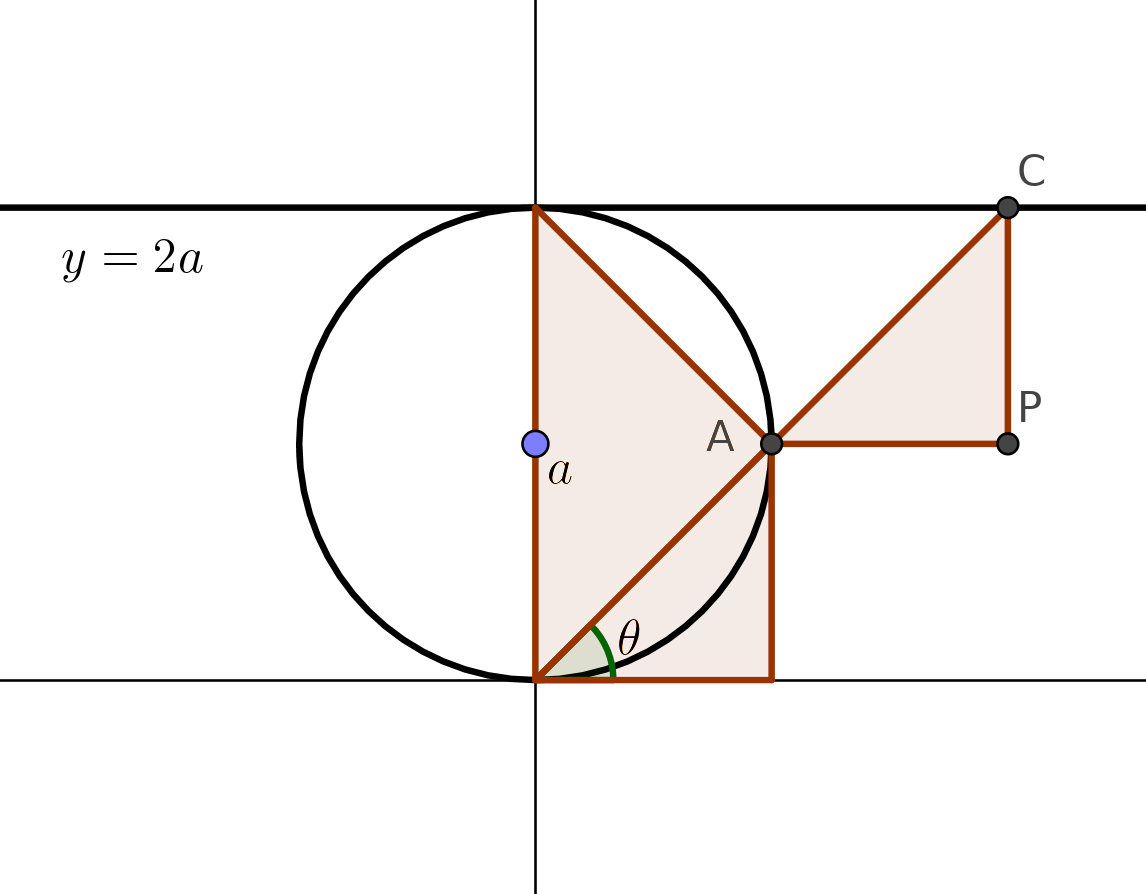
\includegraphics[width=0.5\textwidth]{agnesi-geom}
            \end{center}
  \question A particle moves through space over time; the position of the particle at time $ t $ is
            given by $ (3\sin t, 2\cos t) $ ($ 0 \leq t < 2\pi $).
            \begin{parts}
              \parA What is the component of the acceleration of the particle in the $ x $ direction at $ t = \pi/4 $?
              \parA At what times is the particle stationary in the $ x $ direction?
              \parM Is the particle ever momentarily totally stationary?
            \end{parts}
  \questioE Find the rightmost point on the curve $ x = t - t^6 $, $ y = e^t $.
  \questioE For which values of $ t $ is the curve $ x = \cos 2t $, $ y = 3\cos t $ concave up?
  \questioS Show that the curve $ \gamma : t \mapsto (\cos t, \sin t \cos t) $ has two tangents at (0,0)
            and find their equations.
  \questioS Scholarship 2000: The piriform is the curve defined by the equation $ 16y^2 = x^3(8-x) $ where $ x \geq 0 $.
    \begin{parts}
      \part Show that
            \begin{displaymath}\begin{cases}
              x = 4(1 + \sin \theta)\\
              y = 4(1 + \sin \theta)\cos \theta.
            \end{cases}\end{displaymath}
            are parametric equations for the piriform.
      \part Find $ \od{y}{x} $ in terms of $ \theta $, and show that $ \theta = \frac{\pi}{6} $ is a stationary point of the curve.
    \end{parts}
  \questioO We define a surface $ C $ parametrically in terms of two parameters, $ t $ and $ \theta $:
            \begin{displaymath}
              (x,y,z) = (t, t \cos \theta, t \sin \theta).
            \end{displaymath}
    \begin{parts}
      \part Show that the Cartesian equation for this surface is $ x^2 = y^2 + z^2 $. (This is a cone.)
      \part Show that the intersection between $ C $ and the plane $ z = 2 $ is a hyperbola.
      \part For what angle $ \alpha $ does the intersection between $ C $ and the plane parametrically defined by
            \begin{displaymath}
              (x,y,z) = (u\tan \alpha + 1, u, v)
            \end{displaymath}
            (for parameters $ u $ and $ v $) become a parabola? (Hint: $ x = y \tan \alpha + 1 $, and $ z $ is arbitrary.)
    \end{parts}
\end{questions}
\end{document}
